\document[./main_hagedorn.tex]{subfiles}
\usepackage{amsmath}
\usepackage{pgfplots}
\pgfplotsset{compat=1.11}
\begin{document}
\subsection{Numerical/Algorithmic implementation}
\begin{figure}[h!]
    \centering
    \incfig{recursion-impleentation}
    \caption{recursion impleentation}
    \label{fig:recursion-impleentation}
\end{figure}
\textbf{NOTE THAT THE SECOND TERM IS ZERO FOR K=0}
\textcolor{red}{I STILL ACTUALLY NEED TO MAKE SURE THAT 
THIS APPROACH WOULD WORK WITH EVOLUTION OF THE COEFFICIENTS, 
WHICH I AM ACTUALLY NOT SURE OF AT THE MOMENT: ALSO ARE YOU SURE
APPLYING THE RECURSION RELATION WOULD NOT GIVE YOU JUST ANOTHER 
WAY OF OBTAINING THE COEFFICIENTS OF THE POLYNOMIALS?}
There are two approaches that we can consider with regards 
to the numerical implementation: \textbf{static} and \textbf{adaptive}.
In the static approach the basis set is fixed at all times while for the 
adaptive approach basis vectors are added until the L2 norm is within some 
prescribed tolerance of 1. We investigate the latter approach together 
where the index set is the hyperbolic cross set 
\textcolor{red}{To do:
\begin{itemize}
  \item Understand why the hyperbolic is a better choice...
  \item Everything should be in \cite{lubichQuantumClassicalMolecular2008}
    including proof
\end{itemize}}
At the moment we only report the definition. The hyperbolic 
multi-index set 
$\mathcal{K}(K) := 
\left\{ k \in \mathbb{N}^d: \prod_{n=1}^d (1 + k_n) \leq K \right\}$ with  $K \in \mathbb{N}$. 
Because of the recurrence relation it makes sense to 
consider the cube (Lubich proposes hyperbolic set...)
\subsubsection{Static}
Here, we fix the basis set $\mathcal{K} \subset \mathbb{N}$ throughout 
the dynamics. This means that each time step we need to build the block 
matrix.
\\
In the case of a static basis set throughout the dynamics, we can consider 
pre-computing all higher order cross terms moments involving $\varphi_{00}$
or compute them as we go along when needed. The latter approach is definitely 
the one to take in the adaptive case.
\\
\\
Filling the first diagonal entry of $\bm{F}$
is straightforward
\begin{equation}
  \begin{split}
    \bm{F} = 
    \left[
          \begin{array}{c@{}c@{}c}
            F_{00}
            &
            \left[
             \begin{array}{c}
               \dots                        &
            \end{array}
          \right]
            \\
           \left[
             \begin{array}{cc}
               \dots                            \\
            \end{array}
          \right] 
            & 
           \left[
             \begin{array}{cc}
               \dots                            \\
            \end{array}
          \right] 
            & \dots \\ 
            \left[\begin{array}{ccc}
               \dots                           \\
            \end{array}\right] & 
           \left[
             \begin{array}{cc}
               \dots                            \\
            \end{array}
          \right] 
\\
          \dots & \dots   
      \end{array}\right]
  \end{split}
\end{equation}
Then, we can proceed filling $\bm{F}$ along the columns, 
i.e. fix $l=0$, which is in analogy to moving along the  
axes on the n-dimensional lattice through the recurrence 
relation. Let $k = (0,...,0)$ and $\langle j \rangle = (0,...,1,...,0) $
In order to compute $F_{00 + \langle j \rangle0}$ I need 
$\langle (x - q)_j \varphi_0, W \varphi_0$, the first moment.
\begin{equation}
  \begin{split}
    \bm{F} = 
    \left[
          \begin{array}{c@{}c@{}c}
            F_{00}
            &
            \left[
             \begin{array}{c}
               \dots                        &
            \end{array}
          \right]
            \\
           \left[
             \begin{array}{cc}
               F_{00 + \langle j \rangle 0}  \\
            \end{array}
          \right]_{j=1}^d
            & 
           \left[
             \begin{array}{cc}
               \dots                            \\
            \end{array}
          \right] 
            & \dots \\ 
            \left[\begin{array}{ccc}
               \dots                           \\
            \end{array}\right] & 
           \left[
             \begin{array}{cc}
               \dots                            \\
            \end{array}
          \right] 
\\
          \dots & \dots   
      \end{array}\right]
  \end{split}
\end{equation}
We can now move one step more along the axes of the d-dimensional 
lattice to compute 
$F_{00 + \langle j \rangle 0 + \langle j \rangle 0}$
where we now need the moments 
$\left \langle (\bm{x} - \bm{q})_{j}\varphi_1, W \varphi_0 \rangle \right)_{j=1}^d$
which need the cross terms moments
$\langle (\bm{x} - \bm{q})_j(\bm{x} - \bm{q})_i \varphi_0, W \varphi_0  \rangle $ 
and need to figure out more generally about $F_{00 + \sum_{i=1}^n\langle j  \rangle0}$ for 
some $n$.
\begin{equation}
  \begin{split}
    \bm{F} = 
    \left[
          \begin{array}{c@{}c@{}c}
            F_{00}
            &
            \left[
             \begin{array}{c}
               \dots                        &
            \end{array}
          \right]
            \\
           \left[
             \begin{array}{cc}
               F_{00 + \langle j \rangle 0}  \\
            \end{array}
          \right]_{j=1}^d 
            & 
           \left[
             \begin{array}{cc}
               \dots                            \\
            \end{array}
          \right] 
           \\ 
            \left[\begin{array}{ccc}
                F_{00 + \langle j \rangle 0 + \langle j \rangle 0}  \\
            \end{array}\right]_{j=1}^d 
            & 
           \left[
             \begin{array}{cc}
               \dots                            \\
            \end{array}
          \right] 
\\
          \dots & \dots   
      \end{array}\right]
  \end{split}
\end{equation}
Since the block matrix is Hermitian/self-adjoint and we have 
built the first column, we have implicitly built the first row.
\begin{equation}
  \begin{split}
    \bm{F} = 
    \left[
          \begin{array}{c@{}c@{}c}
            F_{00}
            &
            \left[
             \begin{array}{cccc}
               \overline{F_{00 + \langle j \rangle 0}}  &
            \end{array}
          \right]_{j=1}^d
            \\
           \left[
             \begin{array}{cc}
               F_{00 + \langle j \rangle 0}  \\
            \end{array}
          \right]_{j=1}^d 
            & 
           \left[
             \begin{array}{cc}
               \dots                            \\
            \end{array}
          \right] 
             \\ 
            \left[\begin{array}{ccc}
               F_{00 + \langle j \rangle 0 + \langle j \rangle 0}  \\
           \end{array}\right]_{j=1}^d
            & 
           \left[
             \begin{array}{cc}
               \dots                            \\
            \end{array}
          \right] 
\\
          \dots & \dots   
      \end{array}\right]
  \end{split}
\end{equation}
Now we can fill in the 2nd column
\begin{equation}
  \begin{split}
    \bm{F} = 
    \left[
          \begin{array}{c@{}c@{}c}
            F_{00}
            &
            \left[
             \begin{array}{cccc}
               \overline{F_{00 + \langle 1 \rangle 0}}  &
               \overline{F_{00 + \langle 2 \rangle 0}}  &
               \dots                        &
             \overline{F_{00 + \langle d \rangle 0}} & 
            \end{array}
          \right]
            \\
           \left[
             \begin{array}{cc}
               F_{00 + \langle 1 \rangle 0}  \\
               F_{00 + \langle 2 \rangle 0}  \\
               \dots                            \\
               F_{00 + \langle d \rangle 0}  \\
            \end{array}
          \right] 
            & 
           \left[
             \begin{array}{cc}
               F_{01 + \langle 1 \rangle 0}  \\
               F_{01 + \langle 2 \rangle 0}  \\
               \dots                            \\
               F_{01 + \langle d \rangle 0}  \\
            \end{array}
          \right] 
            & \dots \\ 
            \left[\begin{array}{ccc}
               F_{10 + \langle 1 \rangle 0}  \\
               F_{10 + \langle 2 \rangle 0}  \\
               \dots                           \\
               F_{10 + \langle d \rangle 0}  \\
            \end{array}\right] & 
           \left[
             \begin{array}{cc}
               F_{11 + \langle 1 \rangle 0}  \\
               F_{11 + \langle 2 \rangle 0}  \\
               \dots                            \\
               F_{11 + \langle d \rangle 0}  \\
            \end{array}
          \right] 
\\
          \dots & \dots   
      \end{array}\right]
  \end{split}
\end{equation}
%%%%%%%%%%%%%%%%%%%%%%%%%%%%%%%%%%%%%%%%%%%%%%%%
%
%
%   ADAPTIVE APPROACH FOR THE WAVEPACKETS
%
%
%
%%%%%%%%%%%%%%%%%%%%%%%%%%%%%%%%%%%%%%%%%%%%%%%
\subsubsection{Adaptive}
Fixing the basis set throughout the dynamics might not 
be such a good idea especially one case about preserving 
conserved quantities such as the norm within some prescribed 
tolerance $\mathcal{TOL}$. One may consider a larger set than 
necessary at time zero to begin with but requires some educated 
guessing about how many basis function are necessary. It would more 
convenient to consider an adaptive approach. 
\begin{enumerate}
  \item Decompose initial condition at time zero by 
    augmenting the set $\mathcal{K}$ with basis functions until 
    $|\sum_{k \in \mathcal{K}} |c_{k}|^2  - 1| <= \mathcal{TOL}$
  \item When updating coefficients/projecting the transmitted wavepacket
    repeat at the same process as in 1 perhaps filling up the set using the 
    unit cube or this hyperbolic set.
\end{enumerate}
\textbf{Example: 1d}
\\
\begin{figure}[ht]
    \centering
    \incfig{integral_recursion}
    \caption{Integral recursion: d=1}
    \label{fig:integral_recursion}
\end{figure}
\\
(the blue denotes the things we have to compute)
(enphasise that one of the terms in the recursion relation 
will have always been pre-computed - but do we use it anywhere else)
\\
Also othe than the moments you will have access to all the results 
since you need to then exponentiate the matrix
\\
Let us first start by fixing $l=0$ and understand how the recursion for 
$\langle \varphi_k, W \varphi_0 \rangle$ unfolds so as to better the 
pattern (also translate so that 
$q=0$). 
\\
\textcolor{blue}{$\langle \varphi_0, W \varphi_0 \rangle$} (given)
\\
$\langle \varphi_1, W \varphi_0 \rangle$ $\leftarrow$  
\textcolor{blue}{$\langle x \varphi_0, W \varphi_0 \rangle$}
(i.e. the first "moment" of the previous one)
\\
$\langle \varphi_2, W \varphi_0 \rangle$ 
$\leftarrow$  
\textcolor{violet}{$\langle \varphi_0, W \varphi_0 \rangle$},
$\langle x \varphi_1, W \varphi_0 \rangle$
$\leftarrow$  
\textcolor{blue}{$\langle x^2 \varphi_0, W \varphi_0 \rangle$}
\\
$\langle \varphi_3, W \varphi_0 \rangle$ 
$\leftarrow$  
\textcolor{violet}{$\langle \varphi_1, W \varphi_0 \rangle$},
$\langle x \varphi_2, W \varphi_0 \rangle$
$\leftarrow$  
\textcolor{violet}{$\langle x \varphi_0, W \varphi_0 \rangle$},
$\langle x^2 \varphi_1, W \varphi_0 \rangle$
$\leftarrow$  
\textcolor{blue}{$\langle x^3 \varphi_0, W \varphi_0 \rangle$}
\\
$\langle \varphi_k, W \varphi_0 \rangle$ 
$\leftarrow$  
\textcolor{violet}{(already computed staff)}
\textcolor{blue}{$\langle x^k \varphi_0, W \varphi_0 \rangle$}
\\
Still to answer the question of whether I use the moments at 
any other stage --- use Hermitian property...
\\
\\
presumably k 0 involves x2 moment -> check - already computed
\\
\\
This means I need to focus only on the integrals 
involving $\varphi_0$
\\
\\
Now it obviously does make perfect sense. But then is there
really an advantage...? because essentially you are 
computing the integral of a polynomial against a gaussian 
but the polynomial is simplified essentially.. I suppose it 
would depend on whether you can approximate these integral more 
easily since you do know the "polynomials" in your integral...
\\
Essentially all it is is that we do know the monomials explicitly, 
all that has be done really is "hide" the constants and the 
rescaling (I mean they are polynomials)
\subsection{Approximation of F and higher order cross terms}
\textcolor{red}{Is the inner product invariant to translations...?}
\\
Hence, we are interested in computing the following integrals 
involving $\varphi_0^\epsilon$. Translate center to origin: 
$\bm{y} = \bm{x} - \bm{q}$ 
\begin{equation}
  \begin{split}
    &\left \langle
      \prod_{i = 1}^d \bm{y}^{\alpha_i}_{i} \varphi^\epsilon_{0},
      W(\bm{y} + \bm{q}) \varphi^\epsilon_{0}
  \right \rangle
  = \int_{\mathbb{R}^d}
  \prod_{i = 1}^d \bm{y}^{\alpha_i}_{i} 
  W(\bm{y + q}) |\varphi^\epsilon_0|^2 d \bm{y}
\end{split}
\end{equation}
\textcolor{red}{Questions: Consider the non-quadratic remainder $W(\bm{x})$
of a conical intersection crossing? (I do not think any problems arise if $W$ 
has a spike singularity - this would be crossing is reached)
\begin{itemize}
  \item Suppose $\mathbb{N}^d \ni \alpha = 0_{\mathbb{N}^d}$. Then, for 
    $W$ (what assumptions are needed for the Laplace's method?) nice, the 
    integrand is concentrated around $\bm{q}$ with variance...? 
  \item But how does the integral behave as we consider higher moments? (plot...)
        In particular, does the constant in the error using Laplace's method depend 
        on the index..? You would think it would, so what about 
        consider differentiation but then do I really want to do that...
        \\
        Perhaps, it is easier this way as you would be just looking at product rule 
        rather than introducing a delta and differentiating with respect to it
  \item Could it be streched more in one direction than in another?
  \item Does the approximation get worse with the order of the moments...
  \item Other options: sequence of one dimensional integration, fake 
    derivative, and therefore only one integral..
  \item More precisely, will the constant in the error get worse?
\end{itemize}}
\begin{figure}[h!]
  % GNUPLOT: LaTeX picture with Postscript
\begingroup
  \makeatletter
  \providecommand\color[2][]{%
    \GenericError{(gnuplot) \space\space\space\@spaces}{%
      Package color not loaded in conjunction with
      terminal option `colourtext'%
    }{See the gnuplot documentation for explanation.%
    }{Either use 'blacktext' in gnuplot or load the package
      color.sty in LaTeX.}%
    \renewcommand\color[2][]{}%
  }%
  \providecommand\includegraphics[2][]{%
    \GenericError{(gnuplot) \space\space\space\@spaces}{%
      Package graphicx or graphics not loaded%
    }{See the gnuplot documentation for explanation.%
    }{The gnuplot epslatex terminal needs graphicx.sty or graphics.sty.}%
    \renewcommand\includegraphics[2][]{}%
  }%
  \providecommand\rotatebox[2]{#2}%
  \@ifundefined{ifGPcolor}{%
    \newif\ifGPcolor
    \GPcolortrue
  }{}%
  \@ifundefined{ifGPblacktext}{%
    \newif\ifGPblacktext
    \GPblacktexttrue
  }{}%
  % define a \g@addto@macro without @ in the name:
  \let\gplgaddtomacro\g@addto@macro
  % define empty templates for all commands taking text:
  \gdef\gplbacktext{}%
  \gdef\gplfronttext{}%
  \makeatother
  \ifGPblacktext
    % no textcolor at all
    \def\colorrgb#1{}%
    \def\colorgray#1{}%
  \else
    % gray or color?
    \ifGPcolor
      \def\colorrgb#1{\color[rgb]{#1}}%
      \def\colorgray#1{\color[gray]{#1}}%
      \expandafter\def\csname LTw\endcsname{\color{white}}%
      \expandafter\def\csname LTb\endcsname{\color{black}}%
      \expandafter\def\csname LTa\endcsname{\color{black}}%
      \expandafter\def\csname LT0\endcsname{\color[rgb]{1,0,0}}%
      \expandafter\def\csname LT1\endcsname{\color[rgb]{0,1,0}}%
      \expandafter\def\csname LT2\endcsname{\color[rgb]{0,0,1}}%
      \expandafter\def\csname LT3\endcsname{\color[rgb]{1,0,1}}%
      \expandafter\def\csname LT4\endcsname{\color[rgb]{0,1,1}}%
      \expandafter\def\csname LT5\endcsname{\color[rgb]{1,1,0}}%
      \expandafter\def\csname LT6\endcsname{\color[rgb]{0,0,0}}%
      \expandafter\def\csname LT7\endcsname{\color[rgb]{1,0.3,0}}%
      \expandafter\def\csname LT8\endcsname{\color[rgb]{0.5,0.5,0.5}}%
    \else
      % gray
      \def\colorrgb#1{\color{black}}%
      \def\colorgray#1{\color[gray]{#1}}%
      \expandafter\def\csname LTw\endcsname{\color{white}}%
      \expandafter\def\csname LTb\endcsname{\color{black}}%
      \expandafter\def\csname LTa\endcsname{\color{black}}%
      \expandafter\def\csname LT0\endcsname{\color{black}}%
      \expandafter\def\csname LT1\endcsname{\color{black}}%
      \expandafter\def\csname LT2\endcsname{\color{black}}%
      \expandafter\def\csname LT3\endcsname{\color{black}}%
      \expandafter\def\csname LT4\endcsname{\color{black}}%
      \expandafter\def\csname LT5\endcsname{\color{black}}%
      \expandafter\def\csname LT6\endcsname{\color{black}}%
      \expandafter\def\csname LT7\endcsname{\color{black}}%
      \expandafter\def\csname LT8\endcsname{\color{black}}%
    \fi
  \fi
    \setlength{\unitlength}{0.0500bp}%
    \ifx\gptboxheight\undefined%
      \newlength{\gptboxheight}%
      \newlength{\gptboxwidth}%
      \newsavebox{\gptboxtext}%
    \fi%
    \setlength{\fboxrule}{0.5pt}%
    \setlength{\fboxsep}{1pt}%
\begin{picture}(8620.00,10060.00)%
      \csname LTb\endcsname%%
      \put(4310,9856){\makebox(0,0){\strut{}Integrand}}%
      \put(4310,9633){\makebox(0,0){\strut{}}}%
    \gplgaddtomacro\gplbacktext{%
    }%
    \gplgaddtomacro\gplfronttext{%
      \csname LTb\endcsname%%
      \put(3171,9123){\makebox(0,0)[r]{\strut{}g0(x,y)}}%
    }%
    \gplgaddtomacro\gplbacktext{%
    }%
    \gplgaddtomacro\gplfronttext{%
      \csname LTb\endcsname%%
      \put(7481,9123){\makebox(0,0)[r]{\strut{}g1(x,y)}}%
    }%
    \gplgaddtomacro\gplbacktext{%
    }%
    \gplgaddtomacro\gplfronttext{%
      \csname LTb\endcsname%%
      \put(3171,6720){\makebox(0,0)[r]{\strut{}g2(x,y)}}%
    }%
    \gplgaddtomacro\gplbacktext{%
    }%
    \gplgaddtomacro\gplfronttext{%
      \csname LTb\endcsname%%
      \put(7481,6720){\makebox(0,0)[r]{\strut{}g3(x,y)}}%
    }%
    \gplgaddtomacro\gplbacktext{%
    }%
    \gplgaddtomacro\gplfronttext{%
      \csname LTb\endcsname%%
      \put(3171,4316){\makebox(0,0)[r]{\strut{}g4(x,y)}}%
    }%
    \gplgaddtomacro\gplbacktext{%
    }%
    \gplgaddtomacro\gplfronttext{%
      \csname LTb\endcsname%%
      \put(7481,4316){\makebox(0,0)[r]{\strut{}g5(x,y)}}%
    }%
    \gplbacktext
    \put(0,0){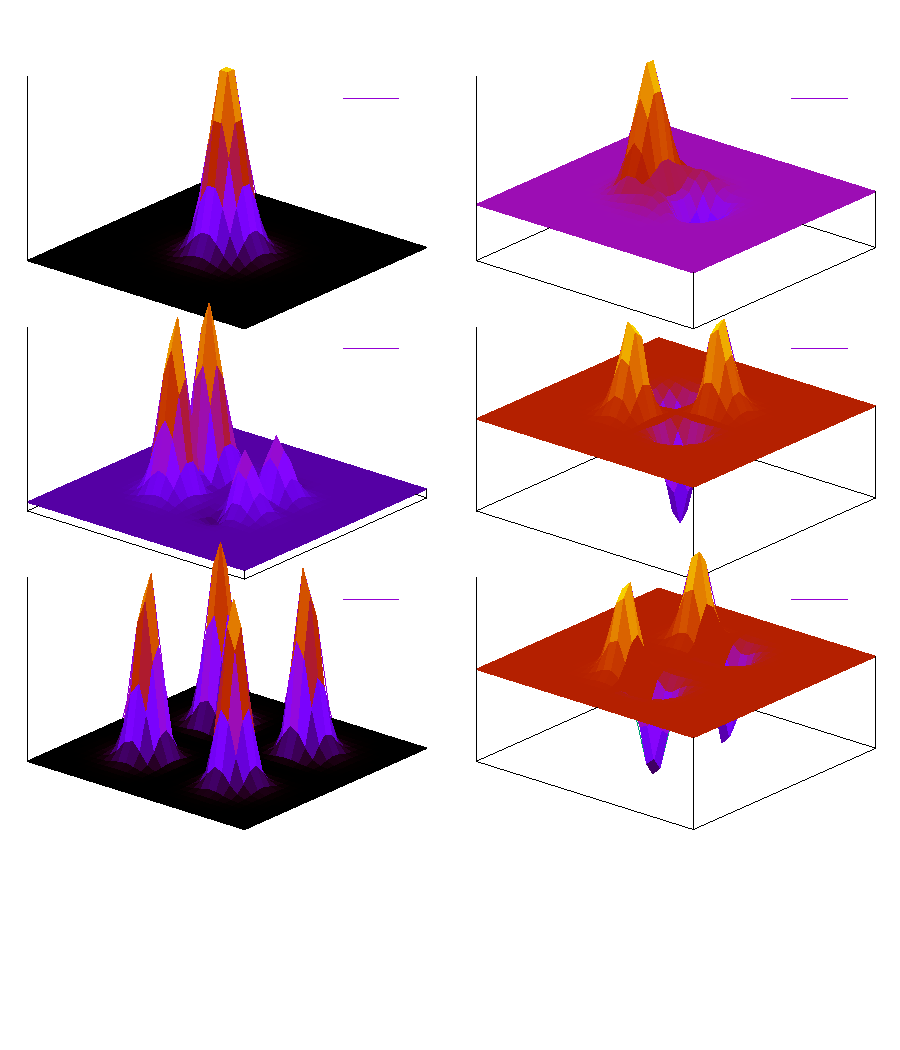
\includegraphics{/home/s1992054/PhD/year-1/hagedorn/plots/gaussian}}%
    \gplfronttext
  \end{picture}%
\endgroup

\end{figure}
\textcolor{red}{Question:
One can approximate the integral using Laplace's method but 
would you diagonalise or not? Diagonalisation requires computation of 
eigenvalues which might not be so convenient.}
where $\alpha$ is an index of powers which, if the sub-basis is fixed 
will be at most $|\alpha| = \sum_{i=1}^d \alpha_i < f(|\mathcal{K}|)$ 
\\
\\
Laplace's method would require quite a few number of terms ? in order 
to give a good error. But derivatives may be expensive to compute? Also, 
wouldn't the number of terms grow factorially with the dimension 
when we have composition of differential operators?
\\
\textbf{Alternative:}
Consider the integral in (1.25). One solution can be as follows: 
\begin{equation}
  \begin{split}
  &\int_{\mathbb{R}^d}\prod_{i = 1}^d \bm{y}^{\alpha_i}_{i} 
  W(\bm{y + q}) 
  e^{-\frac{1}{\epsilon}\bm{y}^T\Im(\bm{C})\bm{y}}
  d \bm{y}
  \\
  &=
  \sqrt{\frac{(2\pi)^d}{\det \Im(\bm{C})}}
  \exp{\left[\frac{\epsilon}{4}\right]}
  \end{split}
\end{equation}
For certain $u(\bm{x})_{s}$, checking the conditions, one can solve the integral 
as follows
\begin{equation}
  \begin{split}
   h 
  \end{split}
\end{equation}
Recall the parameters depend on time. Could this be more efficient than 
numerical integration? Does not look like it?
\end{document}
%The property of Hagedorn wavepackets with respect to the Fourier Transform
%\textcolor{red}{to verify one can interchange integration and summation
%when going from a position to a momentum representation when expressed as
%an infinite sum... dominated convergence theorem...?}

%Equation \eqref{Hagedorn:quadratic:q:p} is just Ehnfrest Theorem for
%quadratic potentials. Then, perhaps something similar for the equations
%below? Then the true result is showing the Gaussian (property preserved)
%with such evolving parameters is a solution.
%
%      Properties from Lemma 1.1 and norm are preserved and therefore the
%      matrix $C$ remains a complex symmetric matrix with positive definite
%      imaginary part in time.
%      \textbf{!!!!} Also in the 1D case should I update the phase of
%      $\varphi_0$ where its initial coefficient is 1?
%  \\
%  \\
%  The set of initial conditions can be extended to include the so-called
%  Hagedorn wave-packets where $\varphi_0$ can be replaced by any $\varphi_k$
%  in the solution of \eqref{Schrodinger} with $\varphi_k$ given by a
%  recurrence relation (instead of involving partial derivives)
%  and $k = (k_1,k_2,...,k_d)$...
%  \\
%  These Hagedorn wave-packets turn out to form a parametric basis for $L^2$.
%  Hence, these will evolve in time when solving \eqref{Schrodinger} as the
%  parameters evolve and vectors are defined recursively for each set of
%  parameter values (I think you might need to evaluate them at each time step
%  in order to adjust the phase coefficients). In other words since the ladder
%  operators depend on $q,p,Q,P$ they will evolve in time. The result about the
%  evolution of the ladder operators is needed to show the $\varphi_k$s do
%  solve \eqref{Schrodinger}
%  \begin{enumerate}
%      \item Lemma 1.1 allows to check the ... property is preserved under the
%          dynamics
%      \item Variational "Galerkin condition": minimise error in the
%          approximate dynamics my minimising the residual between the true
%          time derivative and the approximate one such that it is orthogonal
%          to the subspace spanned by the finite subbasis (careful since the
%          hagedorn wavepackets are eigenvectors of AA and not H)
%      \item $\text{Im}C = (QQ^{*})^{-1}$ is real if properties of Lemma 1.1
%          are satisfied
%      \item Since $\varphi_0$ spans the null-space of $A$, we have that
%          $\varphi_{0-<j>} = \frac{1}{\sqrt{k_j}}A_j\varphi_0 = 0$
%      \item The numerical scheme proposed in Lubich is essentially strang
%          splitting which translates in an update for the parameters given the
%          results of Hagedorn.
%      \item Need to check how the determinant of $Q$ changes for the
%          normalisation property to hold.
%      \item wavelength?
%      \item How would an approximation by sparse grids work? I can't see it
%          when there's a time dependence..? you would have to transport the
%          grid along with it
%      \item what does he mean by "the method is robust in the classical
%          limit"?
%      \item  generalisation form of Gaussian Wavepackets
%          $$
%          u(x,t) = \exp{()}
%          $$
%      \item Compare to Gaussian treated so far: choose $Q(0)=i$, ...
%      \item $q(t)$ - mean position
%      \item $C(t)$ is a $d$-dimensional complex symmetric matrix (why
%          symmetric) with positive definite imaginary part (so that is an
%          exponential DECAYING gaussian)
%      \textbf{can you always factorise it in such a way}?? see Lemma ... for
%      sufficient condition...
%      \item $p(t)$ - mean momentum
%      \item $\zeta(t)$ - has been untreated in the discussion (i think it
%          becomes the $S(t)$? since it is just a phase-factor
%      \item Particularly interested in the role of $C(t), \zeta(t)$
%      \item See
%      \item Lemma 1.1. Another criterion for invertibility of two matrices
%          leads to the aforementioned decomposition and desired property for
%          the imaginary part of $C$. Why does it make sense for this
%          relations? same questions for the converse. must answer! It goes on
%          to shoe this properties are preserved under the proposed equations
%          of motion
%      \item connection always with classical hamiltonian dynamics and the
%          symplectic properties
%      \item are there some continuity properties or such things w.r.t. to the
%          evolution of the matrices?
%      \item (recall orthogonal matrices are invertible where the inverse is
%          the transpose of the matrix)
%      \item Go through proof. Factorization not unique!
%      \item interpretation of the action
%      \item is there an approximation that goes on when splitting the update
%          in the potential between the quadratic and non quadratic term??
%  \end{enumerate}
%
%\subsection{Initial condition:}



%\subsection*{Questions:}
%
%  For the computational investigation, compare w.r.t.
%  \begin{itemize}
%      \item Is there a way of includig phase-effects through the Hagedorn ODE
%          method? What if I try and derive the transition before applying the
%          zeroth unitary operator. No would not have the decoupling to leading
%          order!
%      \item In 1D they are called hermite polynomials? Is there a closed form
%          expression in this case?
%      \item The splitting approach is closer to SS
%  \item Is it possible that $\phi_0 \not \in \text{span}\{\varphi_k : k \in
%      \mathcal{K}\}$?
%  \item If you do not use SS then you ought be careful to use the quadratic
%      approximation to $V$ to preserve which properties..?
%  \item error for the same computational cost
%      \item is there any computational complexity pen and paper comparison one
%          can make?
%      \item dependence on dimensions
%      \item computational cost for a given error (easier to test than the
%          first point suggested)
%      \item i think in the ode method there is definitely a systematic error
%          coming from the approximation by gaussians which is not there in the
%          strang splitting method. On the other hand, for small $\epsilon$
%          and\/or large dimension the strang splitting method simply becomes
%          unfeasible..(although the systematic error might decay quickly with
%          $\epsilon$??) We do not have it for SS in principle since $\Delta_t$
%          can be made arbitrary small??
%      \item eventually comparison with the other mentioned methods but from a
%          mathematical perspective
%  \end{itemize}
%
%  \subsection*{Additional reading}
%  \begin{itemize}
%      \item Hagedorn's original paper
%
%  \end{itemize}

